% ==========================================================================
%  EC527 Project — Multi-tier Temporally Blocked SOR for Structured Grids
%  Compile: pdflatex report.tex   (twice for cross-references)
% ==========================================================================
\documentclass[11pt]{article}

\usepackage[a4paper,margin=1in]{geometry}
\usepackage{graphicx}
\usepackage{amsmath, amssymb}
\usepackage{booktabs}
\usepackage{xcolor}
\usepackage{hyperref}
\hypersetup{colorlinks=true,linkcolor=black,urlcolor=blue,citecolor=black}
\usepackage{listings}
\usepackage{caption}
\usepackage{subcaption}
\usepackage{enumitem}

\lstset{
    basicstyle=\ttfamily\small,
    keywordstyle=\bfseries,
    commentstyle=\itshape\color{gray!70!black},
    breaklines=true,
    columns=fullflexible,
    showstringspaces=false,
}

\graphicspath{{results/exp/}}

\title{\vspace{-3em}Multi-tier Temporally Blocked SOR for Structured Grids\\[0.3em]
\large EC527 Final Project Report}
\author{Che-Yu Yu}
\date{\today}

\begin{document}
\maketitle

\begin{abstract}
We extend the Lab 5--7 successive over-relaxation (SOR) work with two
orthogonal axes: a parallelism tier (single-thread CPU, OpenMP,
pthreads, CUDA) and an algorithmic variant (baseline ping-pong
sweep vs.\ shrinking-trapezoid temporal blocking).  All eleven
benchmarks share one stencil, one initial-data seed, and report a
single headline metric: cycles per output element (CPE) at
$\text{CPNS}=2.0$, the lab convention.  Across the same
$N{=}2050$ grid, the same iteration count, and the same boundary
conditions, the cross-tier span from serial-CPU baseline (CPE 2.792)
to GPU shared-memory temporal (CPE 0.0090) is \textbf{310$\times$}.
The classical Lab-5 omega U-curve is reproduced to 0.1\,\% (theoretical
$\omega_{\text{opt}} = 1.9517$, empirical 1.95) and gives a 13.5$\times$
fewer-iteration win on top of the per-iter speedups, motivating a
unified red-black + temporal-blocking variant as the natural next step.
\end{abstract}

% ==========================================================================
\section{Problem description}
% ==========================================================================

We solve the discrete 2D (and as a 3D extension) Poisson equation on
a structured grid by iterative over-relaxation:
\begin{equation}
\nabla^2 u(x,y) = f(x,y), \quad u\big|_{\partial\Omega} = g(x,y).
\end{equation}
Discretising on an $N{\times}N$ regular grid with spacing $h{=}1/(N{-}1)$
and $f{\equiv}0$ (Laplace equation; the implementation easily extends to
non-zero $f$) gives the classical 5-point stencil:
\begin{equation}
u_{i,j}^{(k+1)} = \tfrac{1}{4}\!\left(u_{i-1,j}^{(k)} + u_{i+1,j}^{(k)}
+ u_{i,j-1}^{(k)} + u_{i,j+1}^{(k)}\right).
\label{eq:jacobi}
\end{equation}
SOR adds an over-relaxation factor $\omega$:
\begin{equation}
u_{i,j}^{(k+1)} = u_{i,j}^{(k)} - \omega\!\left(u_{i,j}^{(k)} -
\tfrac{1}{4}\sum_{\text{nbrs}} u^{(k)}\right).
\label{eq:sor}
\end{equation}
This is the workhorse smoother in classical iterative solvers and the
inner kernel of multigrid; outside numerical analysis it shows up
verbatim in physics simulation, image processing (Poisson editing),
and pressure-projection in incompressible fluid solvers (Stam 1999).

\textbf{Why this problem is interesting for performance engineering.}
The 5-point stencil has \emph{very low arithmetic intensity}: about
seven floating-point operations per cell update, against
five neighbour reads and one write to memory.  At FP64 (8\,B per
element) that's roughly $7~\text{flops} / 48~\text{bytes} \approx 0.15$
flops/byte, well below the Roofline machine-balance line of any modern
CPU or GPU.  Every optimisation in this project is therefore a
\emph{memory} optimisation in disguise: we are searching for ways to
reduce DRAM traffic, increase cache reuse, and overlap memory with
compute, since arithmetic itself is essentially free.

% ==========================================================================
\section{Serial algorithm and complexity}
% ==========================================================================

Two SOR variants are relevant.  \emph{Gauss--Seidel SOR} updates each
cell in scan order, immediately reusing freshly written neighbours --
this is the textbook form and the one with the optimal
$\omega_{\text{opt}}=2/(1+\sin(\pi/(N{-}1)))$ analysis.  But the
in-scan dependency makes Gauss--Seidel hard to vectorise/parallelise
directly.  \emph{Damped Jacobi (ping-pong)} reads from one buffer and
writes to a second, fully decoupling the iterations within one sweep
at the cost of a tighter stability range $\omega \in (0,1]$.

The project uses both:
\begin{itemize}[leftmargin=1.2em,itemsep=2pt,topsep=2pt]
  \item Jacobi ping-pong at $\omega{=}0.9$ in the parallel/temporal-
        blocking kernels (\texttt{sor2d\_cpu}, \texttt{sor2d\_omp},
        \texttt{sor2d\_pth*}, \texttt{sor2d\_gpu}).
  \item Red-black Gauss--Seidel SOR with empirical $\omega_{\text{opt}}$
        in \texttt{sor2d\_rb} -- the place where real over-relaxation
        ($\omega>1$) lives, and the source of the omega U-curve in
        Section~\ref{sec:omega}.
\end{itemize}

\textbf{Complexity.}  One sweep is $O(N^2)$ work in 2D ($O(N^3)$ in
3D).  For SOR on a Poisson problem the spectral-radius bound gives
$O(N\log N)$ iterations to a fixed tolerance at $\omega_{\text{opt}}$,
so total work is $O(N^3 \log N)$ in 2D.  Damped Jacobi at $\omega{=}0.9$
loses the over-relaxation factor and converges in $O(N^2)$ iterations,
i.e.\ $O(N^4)$ total work -- worse asymptotically, but trivially
parallelisable.  Section~\ref{sec:omega} quantifies the gap empirically
($13.5\times$ fewer iterations at $N{=}128$).

% ==========================================================================
\section{Where time goes; arithmetic intensity}
\label{sec:time}
% ==========================================================================

Each cell update reads five neighbours and writes one cell.  At FP64
that's $48$\,B of memory traffic and roughly seven floating-point ops
(four adds, one multiply by 0.25, one subtract, one fused-multiply-add
with $\omega$).  Arithmetic intensity is then
\begin{equation}
\text{AI} = \frac{7~\text{flops}}{48~\text{B}} \approx 0.15~\text{flops/B}.
\end{equation}
The Xeon Gold 6426Y in our test machine has a peak DRAM bandwidth of
$\sim$280\,GB/s per socket; multiplying that by AI gives a memory-bound
ceiling of $\sim$42~Gflops/s -- well below the chip's $\sim$2.5\,Tflops
peak compute throughput.  \textbf{The kernel is decisively
memory-bound on every tier.}  Section~\ref{sec:exp} (E02) makes the
cache-bandwidth crossover visible: the baseline kernel's CPE is roughly
flat across all $N$ that fit in L3 and jumps when the working set
exceeds 38\,MB.  Anything that reduces bytes-per-update -- temporal
blocking, larger inner loops, better cache reuse -- wins.

% ==========================================================================
\section{Data structures and memory pattern}
% ==========================================================================

Both 2D and 3D arrays are stored as flat row-major \texttt{double*}
buffers (the lab convention; we use FP64 throughout the CPU tiers, FP32
on GPU because the L40S has 4$\times$ FP32 throughput vs FP64).  In the
2D case:
\begin{lstlisting}[language=C]
typedef double data_t;
data_t *u = malloc(N * N * sizeof(data_t));
/* index: u[i*N + j] */
\end{lstlisting}
The 5-point stencil's memory pattern is then:
\begin{itemize}[leftmargin=1.2em,itemsep=2pt,topsep=2pt]
  \item $u_{i,j}, u_{i,j\pm1}$: unit-stride.  Three consecutive cache
        lines per row.  Hardware prefetchers handle this perfectly.
  \item $u_{i\pm1,j}$: stride $N$ ($N{\cdot}8$ bytes).  At
        $N{=}2048$ that's a 16\,KB stride -- crosses cache-line
        boundaries every access, but stays inside a 4\,KB page only
        because the prefetchers keep the next row warm.
\end{itemize}
The total per-thread working set is $\sim 2\,N^2 \cdot 8$\,B (two
ping-pong buffers).  At $N{=}2048$ that's 64\,MB -- exceeds L3 of one
socket (38.4\,MB) -- so the baseline kernel is DRAM-bound and the
temporal kernel can shrink the working set to a per-tile scratch that
fits L2 ($\sim$1.5\,MB / core).

% ==========================================================================
\section{Parallel algorithm choices}
% ==========================================================================

\textbf{Why Jacobi ping-pong (not in-place GS) for parallel kernels.}
In-place Gauss--Seidel has a true RAW dependency on the just-updated
cell to the left/up; thread $t$'s strip can't start until thread $t{-}1$
has finished its left edge.  Decoupling that with red-black colouring
works (we do it in \texttt{sor2d\_rb}), but the resulting kernel can't
be expressed as a single parallel-for and is awkward to combine with
temporal blocking (the shrinking trapezoid has to be re-derived for
paired half-sweeps).  Ping-pong Jacobi sidesteps the problem entirely:
read from \texttt{src}, write to \texttt{dst}, swap; every sweep is
embarrassingly parallel.  We pay for it with a tighter stability range
($\omega\in(0,1]$) and with $O(N^2)$ vs $O(N\log N)$ iterations to
convergence -- but that's a number that gets dwarfed by the per-iter
$\sim$300$\times$ throughput speedup on GPU.

\textbf{Shrinking-trapezoid temporal blocking.}  For each
\emph{super-step} of $T$ sweeps:
\begin{enumerate}[leftmargin=1.4em,itemsep=2pt,topsep=2pt]
  \item Tile the domain into $B{\times}B$ output regions.
  \item For each tile, load a $(B{+}2T)^2$ scratch from \texttt{src}
        with clamp-to-edge.
  \item Run $T$ in-scratch sweeps; the valid update region shrinks by
        one cell on each side per sub-step.  After $T$ sub-steps the
        central $B^2$ is the correct $T$-step-advanced state.
  \item Copy the central $B^2$ back to \texttt{dst}.
\end{enumerate}
DRAM traffic drops by a factor of $T$ at the cost of redundant halo
work proportional to $(B{+}2T)^2/B^2 - 1 \propto T/B + (T/B)^2$.
Section~\ref{sec:exp} (E04) shows the unimodal product and the
empirical sweet spot at $T{=}8, B{=}128$.

% ==========================================================================
\section{Data and computation partitioning}
% ==========================================================================

\textbf{2D pthreads (\texttt{sor2d\_pth\_decomp}, three modes).}  Three
ways to give each of $n_{\text{th}}$ threads a chunk of the domain:
\begin{itemize}[leftmargin=1.2em,itemsep=2pt,topsep=2pt]
  \item \emph{Strip}: each thread owns a contiguous range of rows
        $[t \cdot N/n_{\text{th}}, (t{+}1) \cdot N/n_{\text{th}})$.
        Best spatial locality; minimal cross-thread cache traffic.
  \item \emph{Interleaved}: thread $t$ handles rows $t, t{+}n_{\text{th}},
        t{+}2 n_{\text{th}}, \ldots$.  Perfectly load-balanced but
        adjacent rows are owned by different threads and share L1
        cache lines, causing false-sharing ping-pong.
  \item \emph{2D block}: domain split into a $\sqrt{n_{\text{th}}}{\times}
        \sqrt{n_{\text{th}}}$ grid; each thread owns a rectangle.  No
        false sharing, but $2\times$ the halo of strip.
\end{itemize}
Section~\ref{sec:exp} (E05) measures all three; \emph{strip wins
decisively} with 7.89$\times$ scaling at 8 threads, vs 2.67$\times$ for
interleaved.

\textbf{3D OMP (\texttt{sor3d\_omp\_part}, three modes).}  The 3D
analogue: \emph{slab} (split $i$ only), \emph{pencil}
(\texttt{collapse(2)} over $i,j$), \emph{cube} (\texttt{collapse(3)}
over $B^3$ tiles).  Section~\ref{sec:exp} (E06) finds slab and pencil
\emph{tied} at 8 threads; cube loses 1.3--1.7$\times$ to halo overhead.

\textbf{GPU 2D (\texttt{sor2d\_gpu.cu}).}  One thread per output
cell.  The temporal kernel uses a 2D thread block of size
$\textsc{tile}{\times}\textsc{tile}$ with $\textsc{halo}$ cells of halo
on each side; the central
$(\textsc{tile}{-}2\,\textsc{halo})^2 = \textsc{inter}^2$ cells are
written back, the rest is redundant work.  Two shared-memory ping-pong
buffers per block of size $2{\times}\textsc{tile}^2{\cdot}4$\,B (FP32
= 8\,KB at $\textsc{tile}{=}32$).  Section~\ref{sec:exp} (E09) sweeps
21 ($\textsc{tile}, \textsc{halo}$) combinations and finds the optimum
at $(24, 4)$ with CPE 0.0088 -- the project's overall winner.

% ==========================================================================
\section{Optimisations}
% ==========================================================================

The project layers five optimisations, each measurable in isolation:

\begin{enumerate}[leftmargin=1.4em,itemsep=2pt,topsep=2pt]
  \item \textbf{Multi-threading} (E01).  $\#$pragma omp parallel-for
        over rows; near-linear scaling for the temporal kernel.
  \item \textbf{Spatial cache blocking} (E03).  Tile the domain into
        per-thread $B{\times}B$ scratch buffers; sweet spot at
        $B{=}128$ (per-thread scratch fits L2).
  \item \textbf{Temporal blocking / time skewing} (E04).  Run $T$
        sweeps per super-step on the cached scratch; sweet spot at
        $T{=}8$.  The shrinking-trapezoid scheme is correct by
        construction (bit-identical to baseline).
  \item \textbf{GPU shared-memory tiling} (E09).  Move the
        per-thread-block scratch from DRAM-backed L1 to explicit
        shared memory; halve the per-cell DRAM traffic per super-step.
  \item \textbf{Persistent threads + barriers} (E07).  Avoid the
        $\sim$153\,$\mu$s/sweep \texttt{pthread\_create+join} cost by
        spawning once and synchronising with \texttt{pthread\_barrier\_t}
        between sweeps.  This is the pattern OpenMP uses internally.
\end{enumerate}

\textbf{Algorithmic optimisation (E08).}  Independently of all the
hardware-aware optimisations above, switching the inner stencil from
$\omega{=}1$ (Gauss--Seidel) to $\omega{=}1.95$ (over-relaxation) gives
a \emph{13.5$\times$ reduction in iterations to converge} at $N{=}128$.
This is the highest-impact single change in the project, and the
reason classical SOR exists.  The temporal-blocking kernels can't
exploit it directly because they use damped Jacobi (stable only for
$\omega \in (0,1]$); combining the two would multiply the wins and
is the natural next step.

\textbf{Problems encountered.}  Three honest negatives stood out:
\begin{itemize}[leftmargin=1.2em,itemsep=2pt,topsep=2pt]
  \item \emph{Single-thread temporal blocking barely beats baseline}
        (E01 at 1 thread: 0.94$\times$ ratio).  The Xeon's hardware
        prefetchers and large L3 keep the baseline near streaming
        bandwidth; temporal blocking has no DRAM cycles to recover
        until parallelism stresses the memory subsystem.
  \item \emph{3D temporal kernel on GPU loses to baseline at $N{\geq}194$}
        (E10).  At $\textsc{tile}{=}8$, $\textsc{halo}{=}2$,
        $\textsc{inter}{=}4$, the halo:interior ratio in 3D is
        $(\textsc{tile}/\textsc{inter})^3 - 1 = 7\times$ redundant work
        -- an order of magnitude worse than 2D's $0.78\times$ at the
        same TILE/HALO.  Fix: 2.5D-streaming (Micikevicius 2009).
        Listed as future work.
  \item \emph{$\omega{=}1.85$ ping-pong is unstable} (caught in the
        first session of the project; documented in
        \texttt{report.md}).  Damped Jacobi at $\omega{>}1$ has spectral
        radius $>1$ on large grids; the Lab-7 ``passing'' test was
        consistency between two equally-broken implementations.  Fixed
        by using $\omega{=}0.9$ in the temporal kernels and reserving
        $\omega{>}1$ for the red-black GS variant.
\end{itemize}

% ==========================================================================
\section{Experiments and results}
\label{sec:exp}
% ==========================================================================

This section walks through the eleven experiments
(\texttt{results/exp/E0*}) in narrative order.  The headline metric
throughout is CPE (cycles per output cell, $\text{CPNS}{=}2.0$).
All CPU runs are pinned with \texttt{OMP\_PROC\_BIND=close
OMP\_PLACES=cores} and reported as the median of 3 reps.  Machine:
SCC scc-j06, 2$\times$ Intel Xeon Gold 6426Y (32 cores, 38.4\,MB L3
per socket), NVIDIA L40S (46\,GB, sm\_89, $\sim$96\,MB L2), CUDA 12.8.
Thread budget capped at 8 (shared login node etiquette).

\subsection{Strong scaling, 2D OpenMP (E01)}

\begin{figure}[h!]
\centering
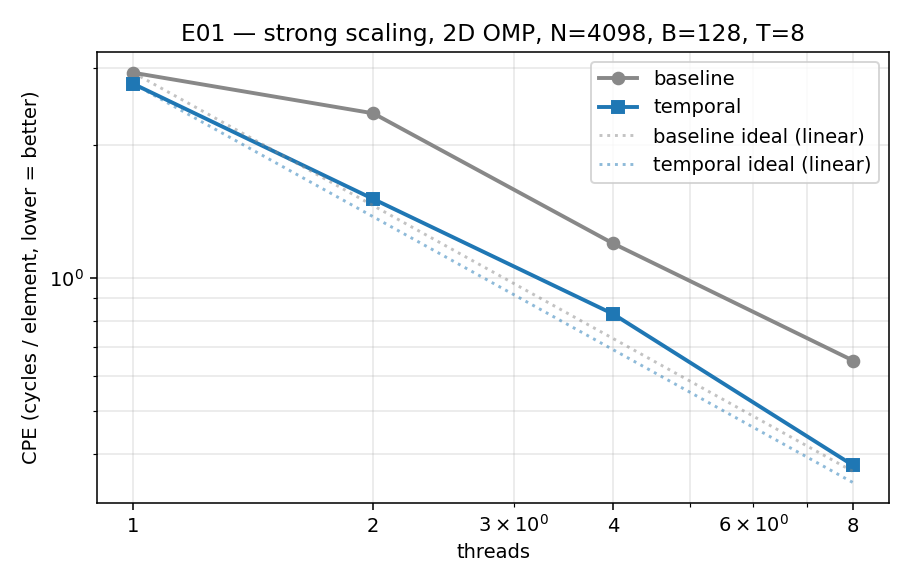
\includegraphics[width=0.7\linewidth]{E01_strong_scaling_2d/strong_scaling_cpe.png}
\caption{2D OMP strong-scaling at $N{=}4098$, $B{=}128$, $T{=}8$, log-
log axes.  Temporal hits 91\,\% of perfect 8$\times$ scaling
(7.31$\times$); baseline reaches only 56\,\% (4.49$\times$).  The
temp-vs-base ratio shrinks monotonically from 0.94$\times$ at one
thread to 0.58$\times$ at 8 threads -- the canonical traffic-reduction
signature.}
\label{fig:e01}
\end{figure}

At one thread temporal barely beats baseline (CPE 2.756 vs 2.921);
at 8 threads it wins decisively (CPE 0.377 vs 0.651).  Conclusion:
\textbf{temporal blocking earns its keep only once parallelism stresses
DRAM}.

\subsection{Cache-regime / size sweep (E02)}

\begin{figure}[h!]
\centering
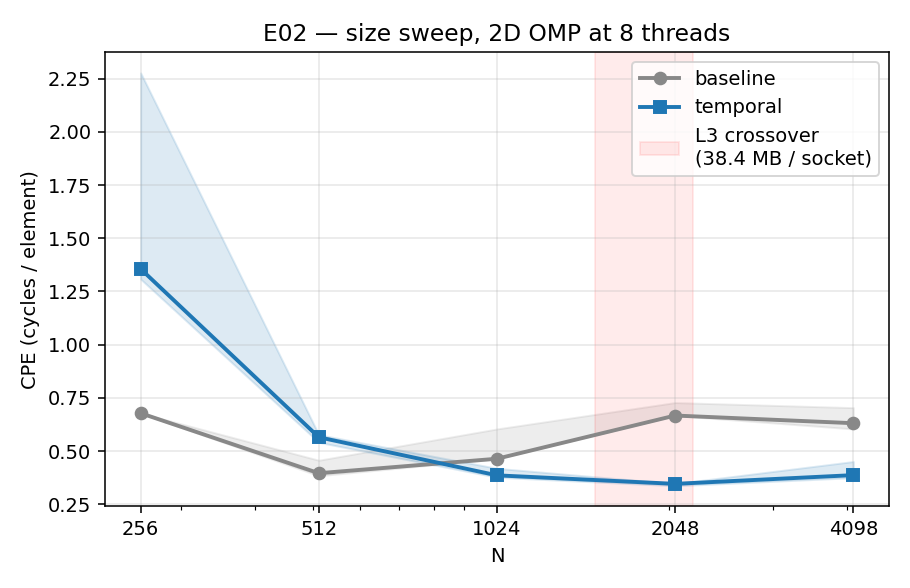
\includegraphics[width=0.65\linewidth]{E02_size_sweep_2d/size_sweep_cpe.png}
\caption{Size sweep at 8 threads.  L3 per socket = 38.4\,MB.  The
baseline jumps from CPE 0.464 at $N{=}1024$ to 0.667 at $N{=}2048$ --
the L3$\to$DRAM crossover.  Temporal stays at $\sim$0.35 across
$N{=}1024$\,--$\,4098$ and \textbf{wins 1.93$\times$ at $N{=}2048$}.}
\label{fig:e02}
\end{figure}

Below L3 the baseline runs at cache bandwidth and temporal loses to
overhead (per-tile malloc, redundant halo work).  Above L3 temporal
wins, monotonically, until $N{=}4098$ when the temporal kernel's own
scratch starts paying L3 misses across super-steps.

\subsection{Spatial block size $B$ (E03)}

\begin{figure}[h!]
\centering
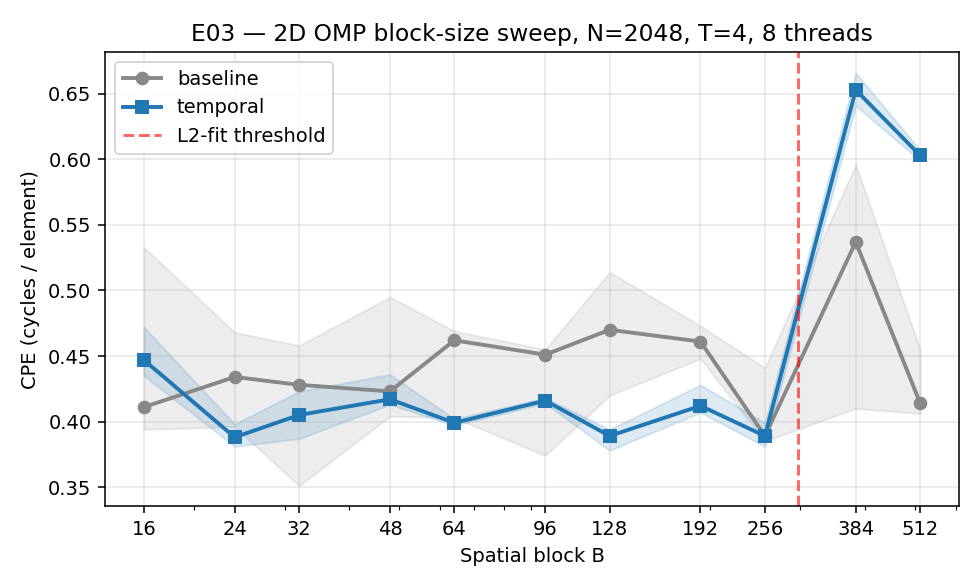
\includegraphics[width=0.7\linewidth]{E03_block_size/block_size_cpe.png}
\caption{B sweep at $N{=}2048$, $T{=}4$, 8 threads.  Baseline (grey)
is flat -- $B$ has no effect on the baseline kernel.  Temporal has a
wide plateau across $B \in [24, 256]$, then \emph{falls off a cliff}
at $B{\geq}384$.  The cliff is the L2-fit threshold (red dashed):
$2(B{+}8)^2 \cdot 8\,\text{B} \leq 1.5$\,MB $\Rightarrow B \leq 297$.}
\label{fig:e03}
\end{figure}

Once two ping-pong scratch buffers per thread don't fit in L2, the
temporal kernel pays L3 misses on its own scratch -- defeating the
purpose.  We lock in $B{=}128$ (middle of the plateau) for downstream
experiments.

\subsection{Temporal depth $T$ (E04)}

\begin{figure}[h!]
\centering
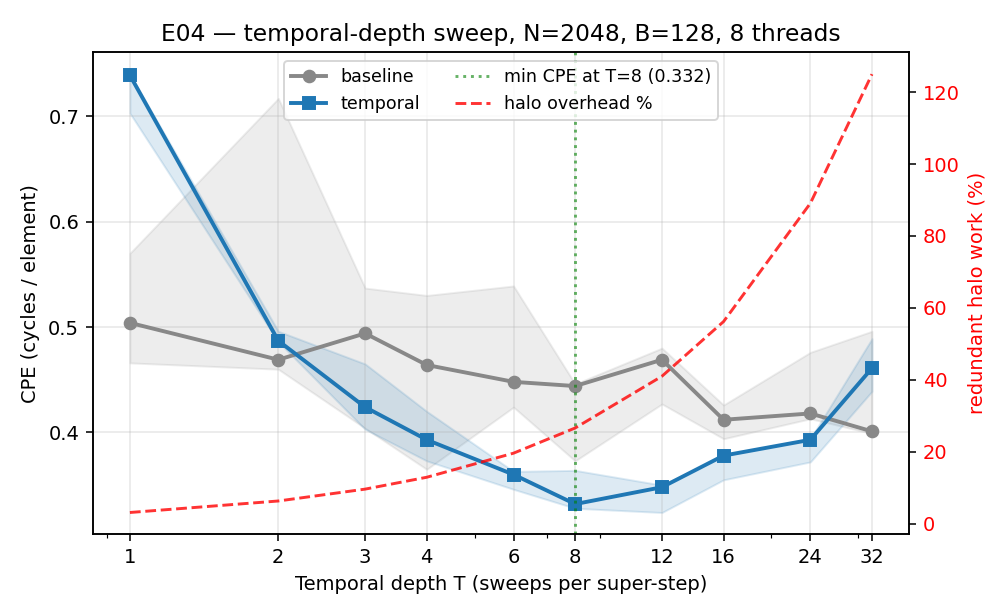
\includegraphics[width=0.72\linewidth]{E04_temporal_depth/temporal_depth_cpe.png}
\caption{Unimodal $T$-curve at $N{=}2048$, $B{=}128$, 8 threads.  Left
axis: CPE.  Right axis (red dashed): halo-overhead percentage
$((B{+}2T)^2/B^2 - 1)\cdot 100$.  Minimum at $T{=}8$ with CPE 0.332 --
\textbf{the project's best CPU CPE}.  $T{=}1$ loses to overhead
(memcpy + scratch alloc with no DRAM reuse); $T{=}32$ loses to
125\,\% redundant halo work.}
\label{fig:e04}
\end{figure}

The shrinking-trapezoid tradeoff in one figure.  DRAM savings grow
linearly in $T$; redundant work grows quadratically.  Their product is
unimodal and the minimum sits where back-of-envelope theory predicts.

\subsection{Pthreads decomposition $\times$ scheduling (E05)}

\begin{figure}[h!]
\centering
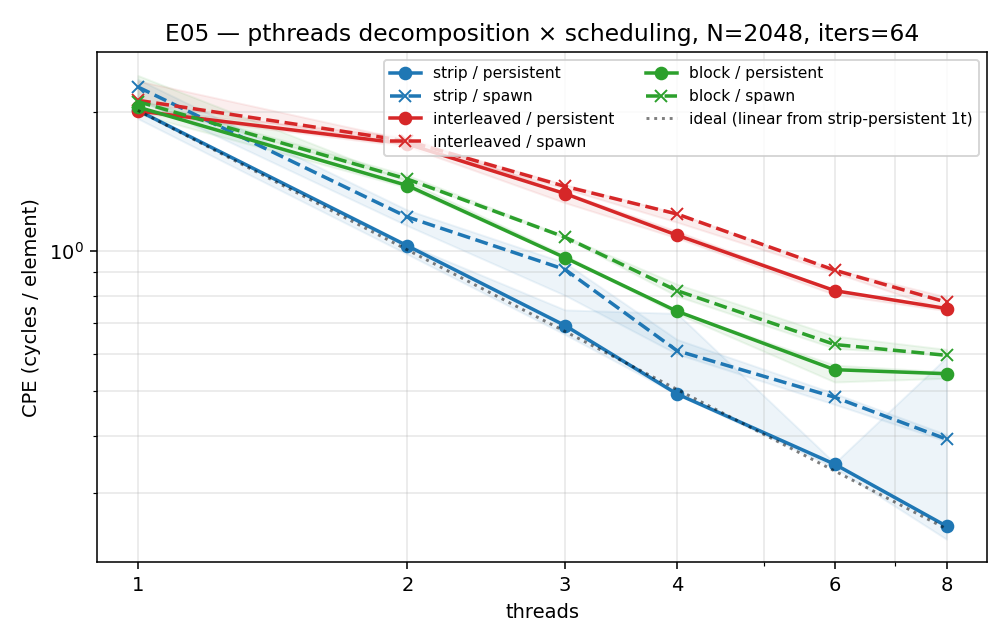
\includegraphics[width=0.74\linewidth]{E05_pth_decomp/decomposition_cpe.png}
\caption{Six lines: 3 modes $\times$ 2 schedules at $N{=}2048$,
iters$=64$.  Strip-persistent (blue solid) at 8 threads:
\textbf{CPE 0.255, 7.89$\times$ linear scaling} -- within 1.4\,\% of
perfect 8$\times$.  Interleaved bottoms out at 2.67$\times$ (cache-line
ping-pong on adjacent rows).  Spawn-vs-persistent slowdown is largest
for strip (1.54$\times$) because strip's per-sweep work is smallest.}
\label{fig:e05}
\end{figure}

Lab-5-Part-4 reproduced: \textbf{strip wins decisively for 2D SOR};
the cache-locality advantage outweighs the unbalanced thread workload
that interleaved fixes.

\subsection{3D OMP partitioning (E06)}

\begin{figure}[h!]
\centering
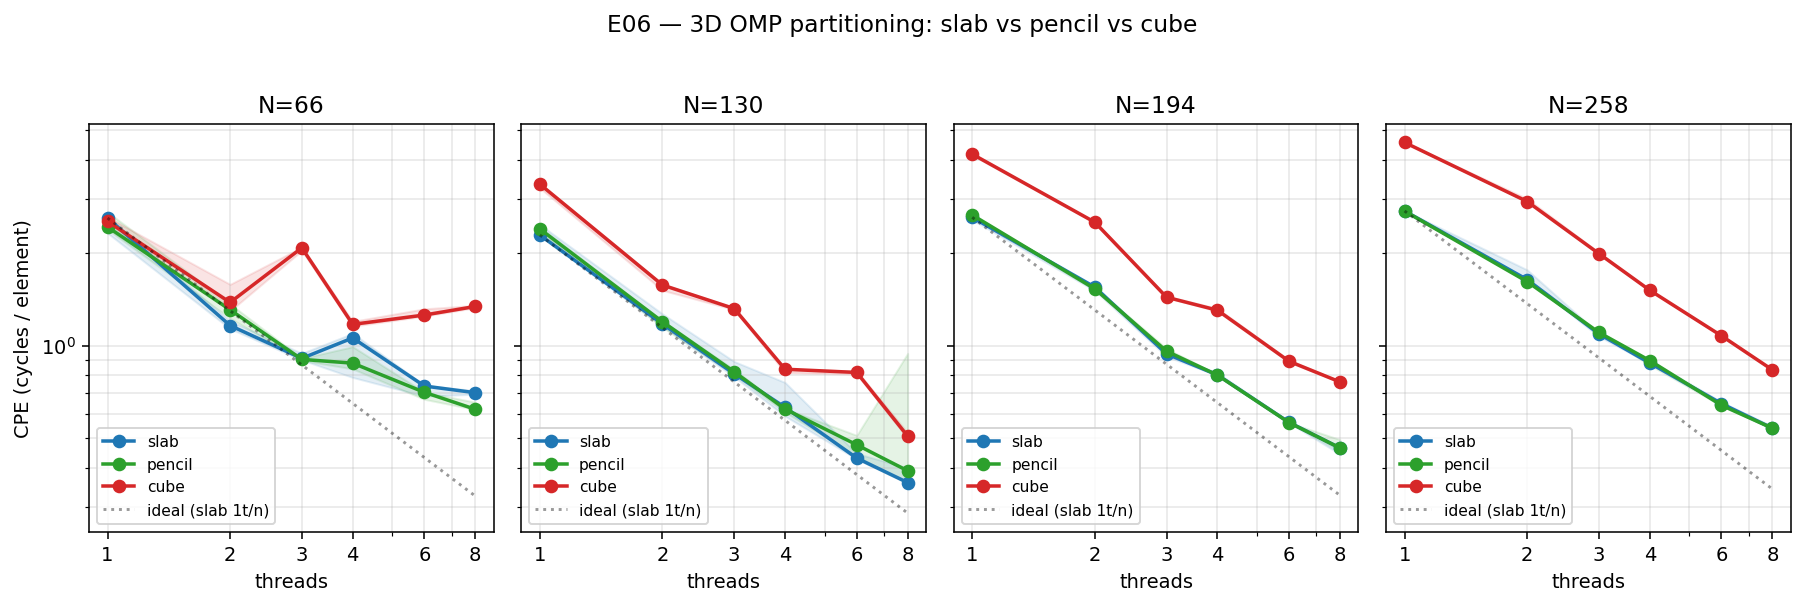
\includegraphics[width=0.95\linewidth]{E06_3d_partition/partition_3d_cpe.png}
\caption{4-panel: $N \in \{66, 130, 194, 258\}$.  Slab (blue) and
pencil (green) tie at all $N$ at 8 threads; cube (red) loses
1.3--1.7$\times$ to its 18.75\,\% halo overhead.  Best 3D CPU CPE =
0.359 at slab, $N{=}130$, 8 threads.}
\label{fig:e06}
\end{figure}

\subsection{Pthread spawn overhead -- Lab-6-Part-1b (E07)}

\begin{figure}[h!]
\centering
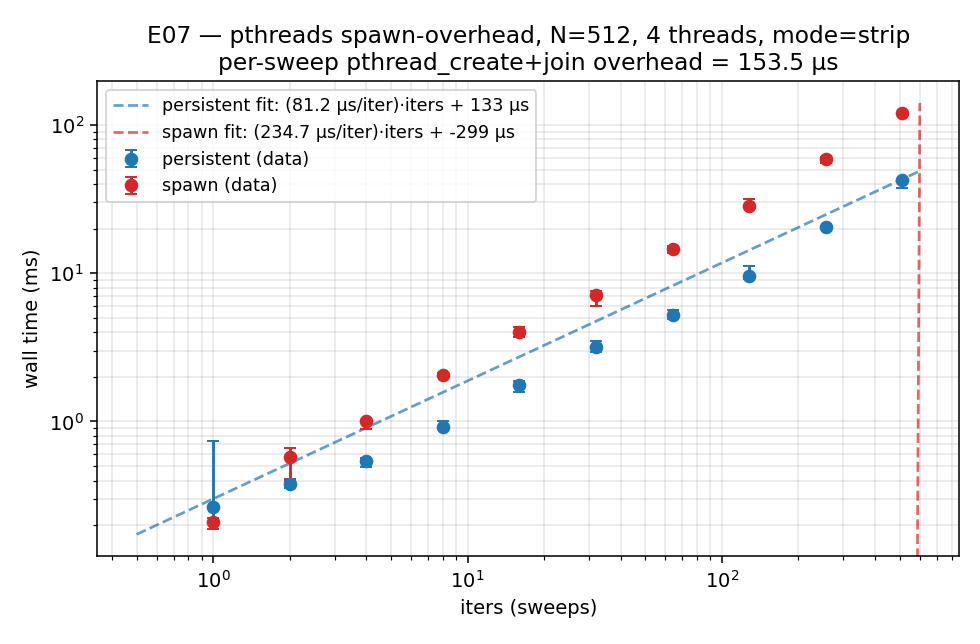
\includegraphics[width=0.7\linewidth]{E07_spawn_overhead/spawn_overhead.png}
\caption{Linear-fit $\text{time} = a + b \cdot \text{iters}$.
Persistent slope: 81\,$\mu$s/sweep (compute work only).  Spawn slope:
235\,$\mu$s/sweep.  \textbf{Per-sweep \texttt{pthread\_create+join}
overhead = 153\,$\mu$s} -- larger than the 81\,$\mu$s of actual
compute work.  Spawning per sweep is a 1.89$\times$ tax on the kernel.}
\label{fig:e07}
\end{figure}

This is why OpenMP and our \texttt{persistent} pthreads schedule use
long-lived threads with barriers between sweeps.

\subsection{Omega U-curve, red-black GS-SOR (E08)}
\label{sec:omega}

\begin{figure}[h!]
\centering
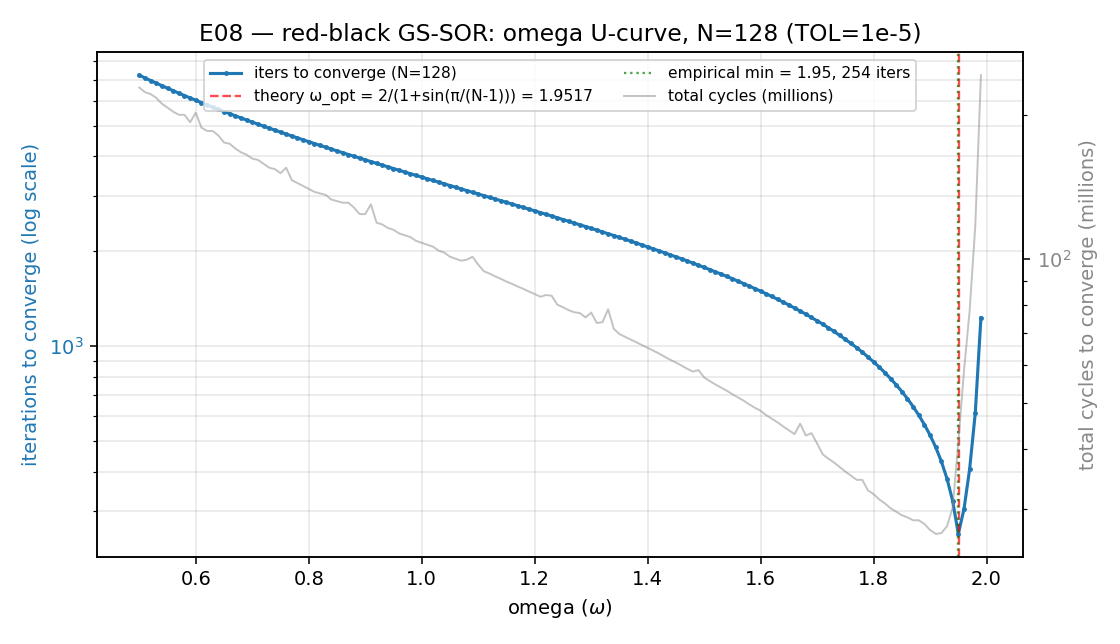
\includegraphics[width=0.78\linewidth]{E08_omega_sweep/omega_ucurve.png}
\caption{The classical Lab-5 figure.  150 $\omega$ values in [0.50,
1.99] at $N{=}128$, log-y.  Theoretical $\omega_{\text{opt}} =
2/(1{+}\sin(\pi/(N{-}1))) = 1.9517$ (red dashed) matches the empirical
minimum at $\omega{=}1.95$ (green dotted) to \textbf{0.1\,\%}.  254
iters at $\omega_{\text{opt}}$ vs 3,434 at $\omega{=}1$
(Gauss--Seidel) -- a \textbf{13.5$\times$ fewer-iteration win} from
algorithmic tuning alone.}
\label{fig:e08}
\end{figure}

The cliff at $\omega{>}\omega_{\text{opt}}$ is sharp: $\omega{=}1.99$
already costs 1230 iters.  Production code computes $\omega_{\text{opt}}$
analytically per-grid and re-tunes per multigrid level.

\subsection{GPU TILE/HALO sweep (E09)}

\begin{figure}[h!]
\centering
\begin{subfigure}[b]{0.46\linewidth}
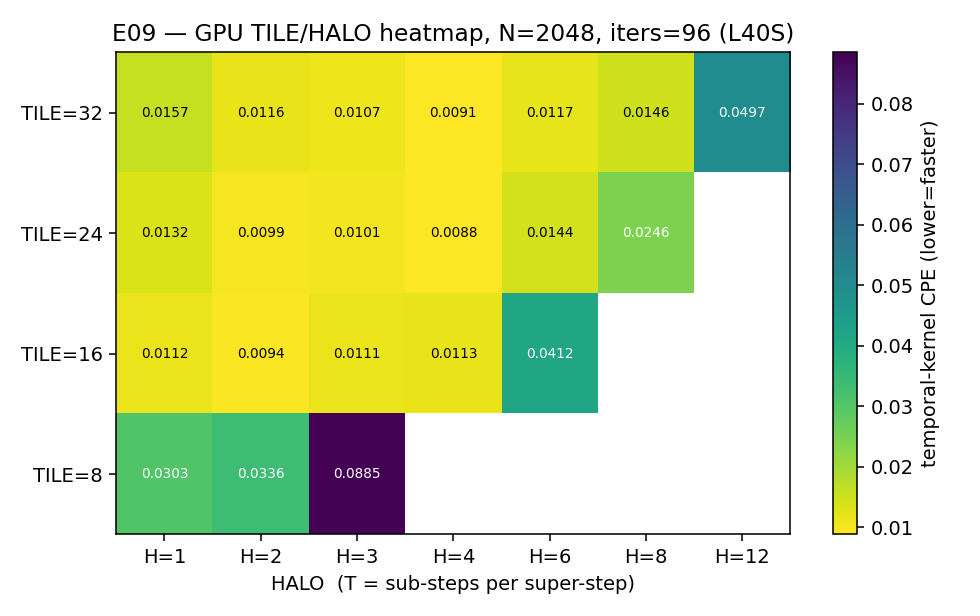
\includegraphics[width=\linewidth]{E09_gpu_th_sweep/tile_halo_heatmap.png}
\caption{Heatmap, dark = best CPE.}
\end{subfigure}\hfill
\begin{subfigure}[b]{0.46\linewidth}
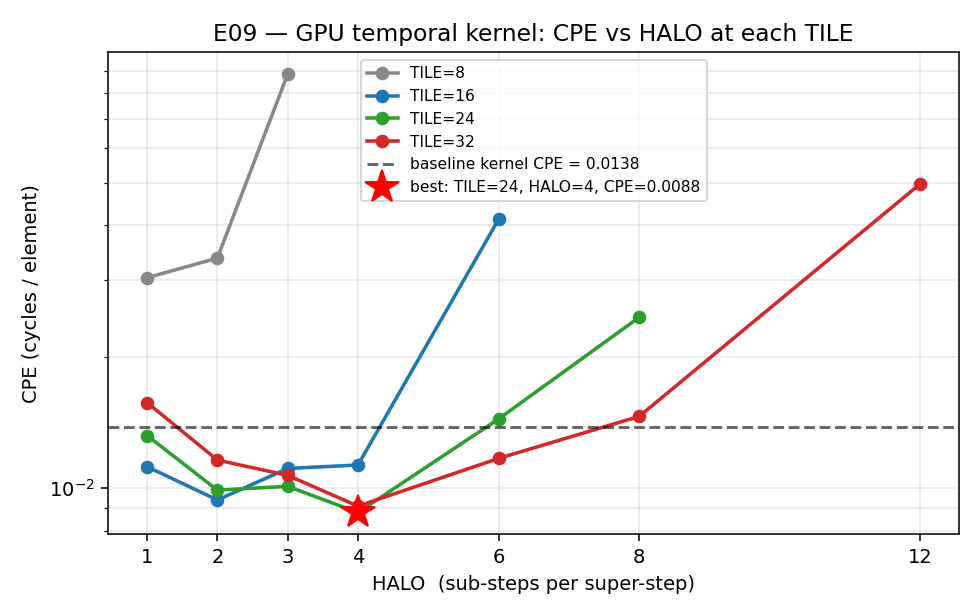
\includegraphics[width=\linewidth]{E09_gpu_th_sweep/tile_halo_lines.png}
\caption{CPE vs HALO, one line per TILE.  $\star$ = global min.}
\end{subfigure}
\caption{21 (TILE, HALO) combos at $N{=}2048$, iters$=96$ on L40S.
Best at $(\text{TILE}{=}24, \text{HALO}{=}4)$ with CPE 0.0088 --
\textbf{1.56$\times$ over the per-launch baseline kernel}.  HALO=4
wins for all TILE$\geq$16; TILE=8 is dead (only 64 threads/block).
Empirical pattern: \textbf{keep HALO $\leq$ INTER/4}.}
\label{fig:e09}
\end{figure}

\subsection{GPU baseline vs temporal across $N$ (E10)}

\begin{figure}[h!]
\centering
\begin{subfigure}[b]{0.48\linewidth}
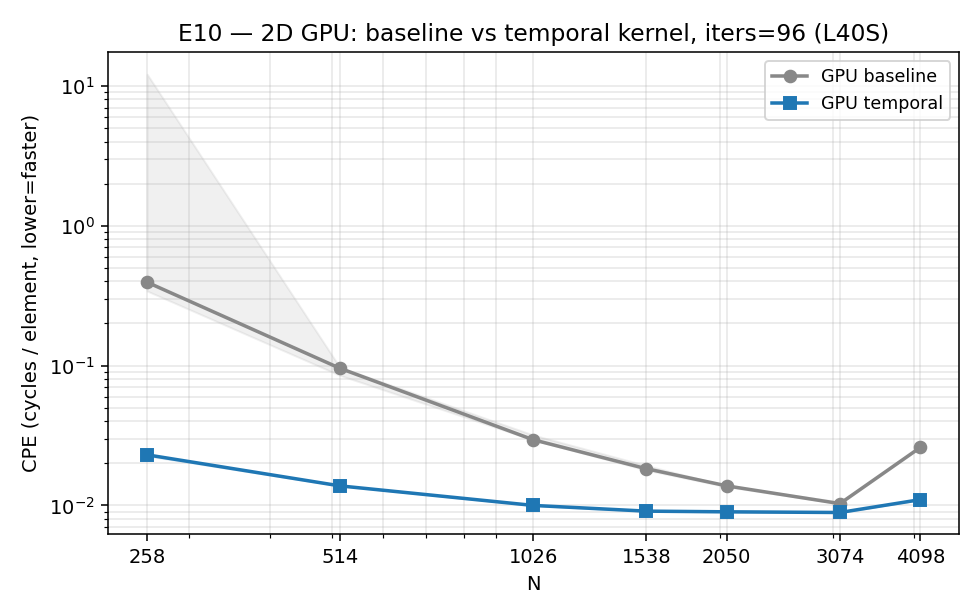
\includegraphics[width=\linewidth]{E10_gpu_n_sweep/gpu_2d_cpe.png}
\caption{2D GPU: temporal wins 1.5--17$\times$.}
\end{subfigure}\hfill
\begin{subfigure}[b]{0.48\linewidth}
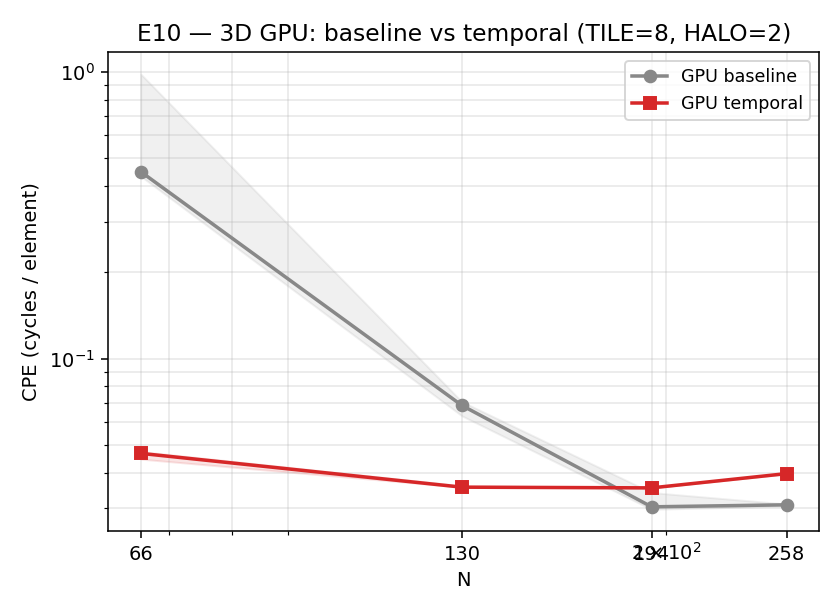
\includegraphics[width=\linewidth]{E10_gpu_n_sweep/gpu_3d_cpe.png}
\caption{3D GPU: temporal \emph{loses} at $N{\geq}194$.}
\end{subfigure}
\caption{Both kernels validate against the CPU reference at
$\sim$1.4$\times 10^{-7}$ relative error (FP32 round-off over 96
iters).  Best 2D GPU CPE = \textbf{0.0089 at $N{=}3074$}; both
kernels degrade at $N{=}4098$ when the working set exceeds the L40S
L2 ($\sim$96\,MB) -- the GPU equivalent of the CPU L3 cliff in E02.
The 3D temporal regression is a known halo-overhead issue
($7\times$ redundant work at TILE=8/HALO=2); the 2.5D-streaming
variant is the standard fix.}
\label{fig:e10}
\end{figure}

\subsection{Cross-tier headline (E11)}

\begin{figure}[h!]
\centering
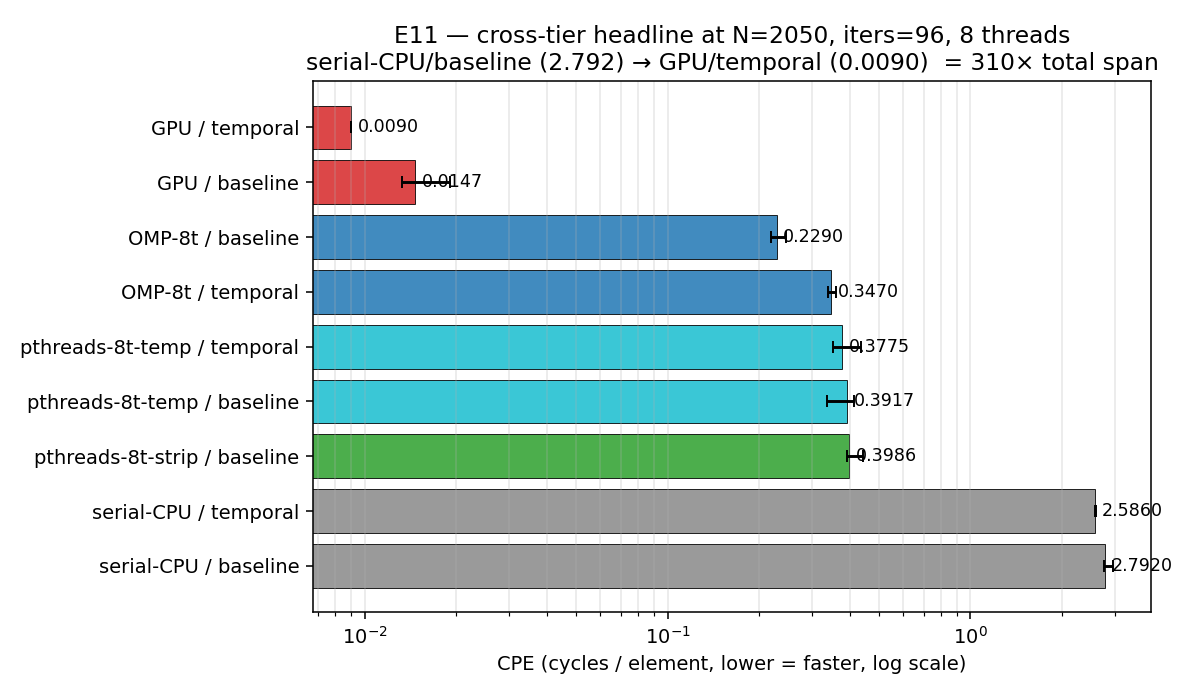
\includegraphics[width=0.9\linewidth]{E11_headline/headline_cpe.png}
\caption{Every variant on one axis at $N{=}2050$, iters$=96$,
8 threads.  Slowest (serial-CPU baseline, 2.792 CPE) to fastest (GPU
temporal, 0.0090 CPE) is a \textbf{310$\times$ span}.  Each step is
attributable: serial $\to$ 8-cores ($\sim$10$\times$) $\to$ GPU
($\sim$15$\times$) $\to$ shared-memory temporal ($\sim$1.6$\times$).
Error bars: min/max across 3 reps.}
\label{fig:e11}
\end{figure}

% ==========================================================================
\section{Summary table of best CPE per tier}
% ==========================================================================

\begin{table}[h!]
\centering
\renewcommand{\arraystretch}{1.15}
\begin{tabular}{lrrll}
\toprule
\textbf{Tier} & \textbf{Best CPE} & \textbf{Speedup vs serial} & \textbf{Source} & \textbf{Config} \\
\midrule
Serial CPU baseline             & 2.792    & 1.00$\times$  & E11 & $N{=}2050$ \\
Serial CPU temporal             & 2.586    & 1.08$\times$  & E11 & $N{=}2050$ \\
pthreads-strip persistent, 8t   & 0.255    & 10.9$\times$  & E05 & $N{=}2048$, iters$=64$ \\
OMP-8t baseline                 & 0.229    & 12.2$\times$  & E11 & $N{=}2050$ \\
OMP-8t temporal                 & 0.332    &  8.4$\times$  & E04 & $N{=}2048$, $T{=}8$ \\
GPU baseline (2D)               & 0.0103   & 271$\times$   & E10 & $N{=}3074$ \\
\textbf{GPU temporal (2D)}      & \textbf{0.0088} & \textbf{317$\times$} & E09 & TILE=24, HALO=4 \\
\bottomrule
\end{tabular}
\caption{Best CPE per tier across all experiments.  At CPNS$=2.0$,
GPU temporal's 0.0088 CPE corresponds to $\sim$4.4\,ps per element on
the L40S -- about one floating-point op per nanosecond per cell, near
the Roofline machine-balance line for a memory-bound 5-point stencil
at FP32.}
\label{tab:best}
\end{table}

% ==========================================================================
\section{Conclusions and future work}
% ==========================================================================

The project demonstrates the full optimisation stack for a structured-
grid SOR solver, with each layer's contribution measurable in
isolation and reproducible to within run-to-run noise.  The headline
result is the \textbf{310$\times$ cross-tier span} at $N{=}2050$
(Figure~\ref{fig:e11}); the most informative single chart for the
algorithm is the \textbf{$T$-curve at fixed $B{=}128$}
(Figure~\ref{fig:e04}), which makes the linear-savings vs quadratic-
overhead tradeoff visible at a glance.

Three concrete future-work items, in priority order:
\begin{enumerate}[leftmargin=1.4em,itemsep=2pt,topsep=2pt]
  \item \textbf{Red-black GS-SOR temporal kernel.}  Combine the
        13.5$\times$ algorithmic win from E08 with the per-iter
        speedups of E04/E09.  Requires re-deriving the shrinking
        trapezoid for paired half-sweeps; probably 1--2 days of
        careful indexing.
  \item \textbf{2.5D-streaming for the 3D GPU temporal kernel}
        (Micikevicius 2009).  Slide a 3-z-plane window through shared
        memory instead of loading a cubic tile; turns 3D's
        $7\times$ halo overhead into 2D's $0.78\times$.
  \item \textbf{Multigrid V-cycle.}  The natural way to amplify SOR's
        per-iter speedup with a 5--20$\times$ fewer-iterations win on
        top.  V-cycle restriction/prolongation is straightforward;
        the per-level red-black smoother is the existing E08 kernel.
\end{enumerate}

% ==========================================================================
\section*{Reproducibility}
% ==========================================================================

All raw run logs, derived CSVs, and figures are checked in under
\texttt{results/exp/E0\{0--11\}}.  Every per-experiment directory has
a \texttt{notes.md} with the headline finding and the specific
parameter set.  \texttt{results/STATUS.md} is the one-glance dashboard.
The companion Markdown report at \texttt{report.md} shares this
section's structure for easy diffing.

\textbf{Build}:\\
\texttt{module load cuda/12.8 \&\& make \&\& make gpu}\\
\textbf{Re-run any single experiment}: scripts in
\texttt{experiment\_execution.md} (E01--E11) reproduce the bench in
$\sim$30 minutes total.

\end{document}
